\section{CW 复形}
\sourcepage{267--268}
我们曾说单纯同调的优点之一是可有效计算。但除最简单的情况外，直接计算所需的工作量通常大到无法手算。即使第 1.7 节计算环面、Klein 瓶的同调时，也没有完全直接计算，而是用了颇具针对性的几何论证，把问题化为较简单的计算。

现在将这些方法整理为计算同调群的系统方法，它既适用于单纯同调，也适用于奇异同调。本节引入比单纯复形更一般的 \textbf{CW 复形}，由 J. H. C. Whitehead 在 [Whi49] 中提出。下一节给每个 CW 复形指定一个\textbf{胞腔链复形}，用它计算底空间的同调。这个链复形比奇异或单纯链复形简单得多。最后一节将用此方法计算实射影空间、复射影空间等的同调。

\entry{定义}{4.12.1}同胚于 $B^m$ 的空间称为 $m$ 维\textbf{胞腔}；同胚于 $\Int B^m$ 的空间称为 $m$ 维\textbf{开胞腔}（open cell）。两种情况下，维数 $m$ 均由空间唯一确定。\translatornote{原书开胞腔定义中的球维数误印为 $n$，应为 $m$。}

\entry{定义}{4.12.2}\textbf{CW 复形}由空间 $X$ 及一族两两不交、并为 $X$ 的开胞腔 $e_\alpha$ 组成，满足：
\begin{enumerate}[label=(\arabic*)]
\item $X$ 为 Hausdorff 空间。
\item 对每个 $m$ 维开胞腔，有连续映射 $f_\alpha:B^m\to X$，把 $\Int B^m$ 同胚地映到 $e_\alpha$，并把 $\Bd B^m$ 映入有限个维数小于 $m$ 的开胞腔之并。
\item 若 $A\cap\overline e_\alpha$ 对每个 $\alpha$ 都在 $\overline e_\alpha$ 中闭，则 $A$ 在 $X$ 中闭。
\end{enumerate}
Whitehead 称 (2) 的有限性为\textbf{闭包有限性}（closure-finiteness）；(3) 表示 $X$ 具有相对于胞腔闭包族的\textbf{弱拓扑}（weak topology）。这两个词就是 CW 中字母 C、W 的来源。

通常记 $\dot e_\alpha=\overline e_\alpha\setminus e_\alpha$。条件 (1)、(2) 蕴含 $f_\alpha(B^m)=\overline e_\alpha$，且 $f_\alpha(\Bd B^m)=\dot e_\alpha$。事实上，由连续性，闭球的像包含于开球像的闭包；另一方面，闭球像紧，在 Hausdorff 空间中闭，并包含 $e_\alpha$，故等于其闭包。边界像与 $e_\alpha$ 不交，因此恰为 $\dot e_\alpha$。

条件 (3) 的逆命题显然成立。映射 $f_\alpha$ 称为胞腔的\textbf{特征映射}（characteristic map）。定义只指定空间及开胞腔族，并不唯一指定特征映射。我们习惯用 $X$ 同时表示 CW 复形及其底空间。

\sourcepage{269}
若开胞腔仅有有限个，称为\textbf{有限 CW 复形}。此时 (2) 的有限性自动成立，(3) 也由其余条件推出：若每个 $A\cap\overline e_\alpha$ 在胞腔闭包中闭，则它在 $X$ 中也闭，有限并 $A$ 因而闭。

有限 CW 复形当然紧。反过来，CW 复形的任意紧子集只能与有限个开胞腔相交；证明留作习题，其中需要闭包有限性。

下面的引理直接来自第 2.8 节关于协调拓扑的一般结果。

\entry{引理}{4.12.3}映射 $f:X\to Y$ 连续，当且仅当每个限制 $f|_{\overline e_\alpha}$ 连续。映射 $F:X\times I\to Y$ 连续，当且仅当每个 $F|_{\overline e_\alpha\times I}$ 连续。

\entry{例}{4.12.4}将环面视为矩形的通常商空间（图 4.12.1）。它有一个二维开胞腔，即矩形内部的像；两个一维开胞腔，即开边的像；一个零维胞腔，即顶点的像。三个定义条件立即成立。
\begin{center}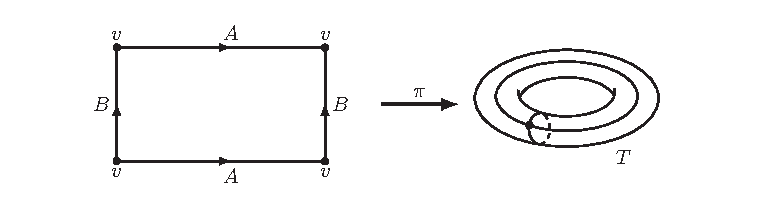
\includegraphics[width=.96\textwidth]{figures/4-12-1.pdf}\\图 4.12.1\end{center}
同样，Klein 瓶也可取各维相同数目的胞腔。实射影平面可取零、一、二维各一个胞腔。更一般地，第 1.7 节习题中的 $n$ 重环面连通和有一个二维胞腔、一个零维胞腔和 $2n$ 个一维胞腔；$n$ 重实射影平面连通和则有一个二维胞腔、一个零维胞腔和 $n$ 个一维胞腔。$k$ 重愚人帽也可取零、一、二维各一个胞腔。

\sourcepage{270}
\entry{例}{4.12.5}将 $B^n$ 的边界压缩为一点所得商空间同胚于 $S^n$，证明留给读者。因此球面可取一个 $n$ 维开胞腔和一个零维胞腔，不需要其他胞腔，见图 4.12.2。
\begin{center}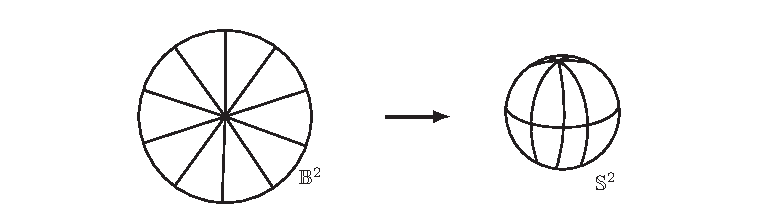
\includegraphics[width=.96\textwidth]{figures/4-12-2.pdf}\\图 4.12.2\end{center}

\entry{例}{4.12.6}条件 (2) 并不要求 $\dot e_\alpha$ 本身等于若干低维开胞腔之并。例如图 4.12.3 的空间在零、一、二维各有一个胞腔，但二维胞腔的边界只包含于低维胞腔之并，并不等于它。
\begin{center}
\includegraphics[width=.96\textwidth]{figures/4-12-3.pdf}\\图 4.12.3\end{center}

\entry{例}{4.12.7}设 $K,L$ 为单纯复形，且 $K$ 局部有限。空间 $|K|\times|L|$ 可取 $(\Int\sigma)\times(\Int\tau)$ 为开胞腔，其中 $\sigma\in K,\tau\in L$。特征映射可取为 $B^m\to\sigma\times\tau$ 的同胚，而且每个闭胞腔的边界是低维开胞腔的有限并。条件 (3) 来自第 2.8 节习题 6，其中用到了 $K$ 的局部有限性。

\sourcepage{271}
\entry{定义}{4.12.8}若 CW 复形的特征映射可取为同胚，且每个 $\dot e_\alpha$ 都等于有限个开胞腔之并，则称为\textbf{正则胞腔复形}（regular cell complex）。这种复形总能三角剖分，使每个闭胞腔是某个子复形的多面体；证明与引理 2.7.3 中对 $|K|\times I$ 的证明类似。

\entry{例}{4.12.9}许多从旧空间构造新空间的方法会保留 CW 结构。例如，两个 CW 复形的乘积 $X\times Y$ 在 $Y$ 局部紧时仍为 CW 复形。粘合空间也常如此：若 $A$ 是 $X$ 的子复形，且 $f:A\to Y$ 把每个 $p$ 维胞腔映入 $Y$ 中维数至多为 $p$ 的开胞腔之并，则称 $f$ 为\textbf{胞腔映射}（cellular map）。此时可证 $X\cup_fY$ 为 CW 复形。

\entry{定义}{4.12.10}设 $Y\subset X$ 为若干开胞腔之并，且每个包含于 $Y$ 的开胞腔，其闭包也包含于 $Y$。下面将证明 $Y$ 在 $X$ 中闭，并且自身构成 CW 复形，称为 $X$ 的\textbf{子复形}。特别地，所有维数至多为 $p$ 的开胞腔之并 $X^p$ 满足这些条件，称为 $X$ 的\textbf{$p$ 维骨架}（$p$-skeleton）。

先验证 $Y$ 的 CW 条件。Hausdorff 性显然；其胞腔的特征映射把整个闭球映入 $Y$，且边界像所碰到的有限个低维胞腔也在 $Y$ 内。只需验证弱拓扑。

设 $B\subset Y$，且 $B\cap\overline e_\alpha$ 对每个在 $Y$ 中的胞腔闭。若 $e_\beta$ 不在 $Y$ 中，则 $Y\cap\overline e_\beta\subset\dot e_\beta$，并包含于有限个在 $Y$ 中的开胞腔 $e_1,\ldots,e_k$ 之并。因此
\[
B\cap\overline e_\beta=\left[\bigcup_{i=1}^k(B\cap\overline e_i)\right]\cap\overline e_\beta.
\]
每个 $B\cap\overline e_i$ 在 $X$ 中闭，故右端闭。由 $X$ 的弱拓扑，$B$ 在 $X$ 中闭，特别在 $Y$ 中闭。因此 $Y$ 具有所需弱拓扑。取 $B=Y$ 还说明 $Y$ 自身在 $X$ 中闭。

\sourcepage{272}
闭包有限性在此证明中至关重要。

\entry{例}{4.12.11}设 $X$ 是平面中的二维单形，取通常拓扑，分解为一个二维开胞腔与边界上无穷多个零、一维胞腔，如图 4.12.4。除条件 (2) 的有限性外，其余条件均成立；条件 (3) 因二维胞腔的闭包等于整个 $X$ 而自动成立。若给边界胞腔之并 $Y$ 赋以相对于各闭胞腔的弱拓扑，$Y$ 自身是 CW 复形，但不具有 $X$ 的子空间拓扑：后者是紧的单形边界，前者却不紧。
\begin{center}
\includegraphics[width=.96\textwidth]{figures/4-12-4.pdf}\\图 4.12.4\end{center}

\entry{定义}{4.12.12}若 CW 复形 $X$ 有三角剖分 $h:|K|\to X$，使每个骨架 $X^p$ 都由维数至多为 $p$ 的子复形三角剖分，则称 $X$ 为\textbf{可三角剖分的 CW 复形}。\footnote{维数条件实际上是多余的，见习题 2。}

前述各例均可三角剖分。下面给出一个不能的例子，证明要用第 4.8 节的局部同调。

\entry{例}{4.12.13}在 $\R^3$ 中，令 $A$ 为正方形与三角形之并，三角形的一条边恰为正方形的对角线 $D$。它是三个三角形共用一条边组成的复形的多面体。在正方形中画一条摆动的弧 $C$，使它与 $D$ 交于一个无限且全不连通的集合，例如 $x\sin(1/x)$ 型曲线。把三维球沿映射 $f:S^2\to C$ 粘到 $A$，其中每条从南极到北极的大圆弧均同胚地映到 $C$，见图 4.12.5。

\sourcepage{273}
\begin{center}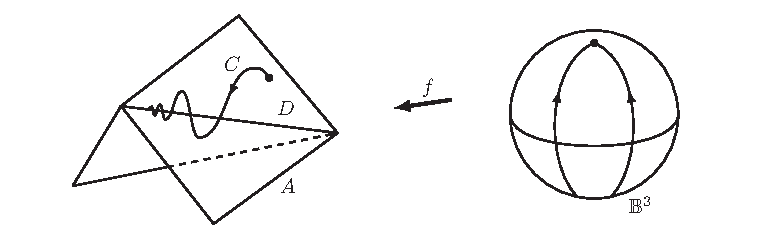
\includegraphics[width=.96\textwidth]{figures/4-12-5.pdf}\\图 4.12.5\end{center}
所得 $X$ 是 CW 复形：取 $A$ 的开单形为低维胞腔，球内部为唯一三维开胞腔 $e^3$。但底空间本身不能三角剖分。

反设 $h:|K|\to X$ 为三角剖分。将 $X$ 写成不交并 $(A\setminus C)\cup C\cup e^3$。若 $x\in e^3$，则它有开三维球邻域，故 $H_3(X,X\setminus\{x\})\cong\Z$；若 $x\in A\setminus C$，有邻域完全包含于二维复形 $A$，故此群由定理 4.8.14 为零。由引理 4.8.10，任一 $h(\Int\sigma)$ 不能同时碰到这两部分。因此每个闭单形的像或包含于 $A$，或包含于 $\overline e^3$。于是 $A,\overline e^3$ 及其交 $C$ 都由 $h$ 三角剖分。

再看 $A$ 自身的局部同调。对角线 $D$ 的内部点 $x$ 满足 $H_2(A,A\setminus\{x\})\cong\Z\oplus\Z$：$A$ 可视为以 $x$ 为顶点、底空间同胚于字母 $\theta$ 形曲线的锥，故由长正合列此群同构于 $H_1(\theta)$。而 $D$ 外的点，局部二维同调或为 $\Z$（三角形内部），或为零。再次由引理 4.8.10，若单形内部像碰到 $\Int D$，便完全包含于 $D$。因此 $D$ 也由 $h$ 三角剖分，进而 $C\cap D$ 亦然。

但 $X$ 紧，所以 $K$ 必为有限复形；其子复形不可能具有无限多个连通分支，而 $C\cap D$ 恰有无限多个分支，矛盾。

把 CW 复形看作由闭球通过商空间粘成，往往很有帮助；也可按这种方式构造新空间，如上例。下面两个定理描述这一过程。CW 复形的\textbf{维数}是胞腔维数的最大值；若无最大值，则称其为无限维。

\sourcepage{274}
\entry{定理}{4.12.14}
\begin{enumerate}[label=(\alph*)]
\item 若 $X$ 为 $p$ 维 CW 复形，则它同胚于把一族闭 $p$ 维球的拓扑和 $\coprod B_\alpha$ 沿连续映射 $g:\coprod\Bd B_\alpha\to X^{p-1}$ 粘到骨架所得的空间。因此 $X$ 正规。
\item 反过来，若 $Y$ 是维数至多为 $p-1$ 的 CW 复形，$g:\coprod\Bd B_\alpha\to Y$ 连续，则将这些闭 $p$ 维球粘到 $Y$ 所得的空间 $X$ 为 CW 复形，$Y$ 为其 $(p-1)$ 维骨架。
\end{enumerate}
\textbf{证明：}(a) 对每个 $p$ 维胞腔取特征映射 $f_\alpha:B^p\to\overline e_\alpha$，令 $B_\alpha=B^p\times\{\alpha\}$。在拓扑和 $E=X^{p-1}\amalg(\coprod B_\alpha)$ 上定义 $\pi:E\to X$：骨架上为包含映射，球上为投影后接 $f_\alpha$。它连续满射，只需证明为商映射。

若 $\pi^{-1}(C)$ 在 $E$ 中闭，则 $C\cap X^{p-1}$ 闭，故与每个低维胞腔闭包的交闭。又对 $p$ 维胞腔，$\pi^{-1}(C)\cap B_\alpha$ 为紧集，其像为 $C\cap\overline e_\alpha$，故在 Hausdorff 空间 $X$ 中闭。由弱拓扑，$C$ 闭，所以 $\pi$ 为商映射。正规性由定理 4.11.3 对 $p$ 归纳得到。

(b) 设 $f:Y\amalg(\coprod B_\alpha)\to X$ 为给定商映射。由 (a)，$Y$ 正规，球的拓扑和也正规，所以定理 4.11.3 说明 $X$ 正规，特别是 Hausdorff。将 $Y$ 认同于其闭像，$f$ 在 $Y$ 上为包含，在球的边界上为 $g$。

取 $Y$ 的原有胞腔及 $e_\alpha=f(\Int B_\alpha)$ 为开胞腔。球内部在拓扑和中开且饱和，限制映射为一一对应的商映射，故为同胚。边界像是 $Y$ 中的紧集，只碰到有限个开胞腔，且这些胞腔维数均小于 $p$，因此条件 (2) 成立。

\sourcepage{275}
最后验证 (3)。若 $C\cap\overline e_\alpha$ 对每个胞腔闭，则 $C\cap Y$ 由 $Y$ 的弱拓扑而闭。对于每个球，
\[
f^{-1}(C)\cap B_\alpha=f^{-1}(C\cap\overline e_\alpha)\cap B_\alpha
\]
闭，因为 $f(B_\alpha)=\overline e_\alpha$，且限制映射连续。因此 $f^{-1}(C)$ 在拓扑和中闭，故 $C$ 在商空间中闭。\hfill$\square$

\entry{定理}{4.12.15}
\begin{enumerate}[label=(\alph*)]
\item 若 $X$ 为 CW 复形，则每个 $X^p$ 在 $X^{p+1}$ 中闭，且 $X$ 是递增骨架族的协调并。因此 $X$ 正规。
\item 反过来，若每个 $X^p$ 为 CW 复形，并为 $X^{p+1}$ 的 $p$ 维骨架，则它们的协调并 $X$ 为 CW 复形，其 $p$ 维骨架恰为 $X^p$。
\end{enumerate}
\textbf{证明：}(a) 若 $C\cap X^p$ 对每个 $p$ 闭，则它与维数至多为 $p$ 的每个胞腔闭包的交都闭。因 $p$ 任意，由弱拓扑 $C$ 闭，故 $X$ 与骨架族协调。各骨架正规，由定理 4.11.6，$X$ 正规。

(b) 若 $p<q$，$X^p\cap X^q=X^p$ 是两者的闭子空间。由引理 4.11.4(b)，协调拓扑存在，各骨架在 $X$ 中闭。每个骨架由上一定理正规，再由定理 4.11.6，$X$ 正规且 Hausdorff。条件 (2) 显然。若 $C$ 与每个胞腔闭包的交闭，则因每个骨架是 CW 复形，$C\cap X^p$ 闭；再由协调拓扑，$C$ 闭。\hfill$\square$

\sourcepage{276}
有时从已有空间出发寻找 CW 结构，如例 4.12.4--4.12.6；有时通过粘合球来构造新空间，如例 4.12.13。以上两个定理给出一般构造，它大大扩展了代数拓扑能有效研究的空间范围。

\subsection*{习题}
\begin{enumerate}
\item 设 $A$ 是 CW 复形 $X$ 的紧子集。
\begin{enumerate}[label=(\alph*)]
\item 证明 $A$ 只与有限个开胞腔相交。证明何处使用了闭包有限性？
\item 证明 $A$ 包含于某个有限子复形。
\end{enumerate}
\item 设三角剖分 $h:|K|\to X$ 在每个骨架上都诱导三角剖分。
\begin{enumerate}[label=(\alph*)]
\item 证明它也在每个胞腔闭包 $\overline e_\alpha$ 上诱导三角剖分。
\item 若 $K_p$ 是剖分 $X^p$ 的子复形，证明其维数至多为 $p$。〔提示：用局部同调群。〕
\end{enumerate}
\item 证明 CW 复形的拓扑紧生成，见第 4.11 节习题 3。
\item 设 $X,Y$ 为 CW 复形，以 $e_\alpha\times e_\beta$ 为乘积的开胞腔。
\begin{enumerate}[label=(\alph*)]
\item 若 $Y$ 局部紧，证明 $X\times Y$ 为 CW 复形。
\item 一般情况下，证明 $X\times_CY$ 为 CW 复形，见第 4.11 节习题 3。
\end{enumerate}
\item 验证正则胞腔复形可三角剖分，使每个闭胞腔是子复形的多面体。
\item 证明 $n$ 维环面为 CW 复形。
\item 证明三维空间中的实心环面为 CW 复形。
\end{enumerate}
